\documentclass[10pt,a4paper,titlepage]{report}
\usepackage[utf8]{inputenc}
\usepackage{amsmath}
\usepackage{amsfonts}
\usepackage{amssymb}
\usepackage{graphicx}
\usepackage{xcolor}
\usepackage{minted}

\newcommand{\HRule}[1]{\rule{\linewidth}{#1}}

\nonstopmode


\begin{document}
{\fontfamily{cmr}\selectfont
\title{ \normalsize \textsc{}
\\ [2.0cm]
\HRule{0.5pt} \\
\LARGE \textbf{\uppercase{Triggers and Exceptions}
\HRule{2pt} \\ [0.5cm]
\normalsize \today \vspace*{5\baselineskip}}
}

\date{}

\author{
	Rwithik Manoj \\
	College of Engineering, Trivandrum \\
	Department of Computer Science and Engineering }

\maketitle
\newpage

\sectionfont{\scshape}

\subsubsection{Create a table customer\_details (cust\_id (unique), cust\_name, address).\newline
Create a table emp\_details(empid(unique), empname, salary).\newline
Create table cust\_count(count\_row).\newline
}
\begin{enumerate}
	\item Create a trigger whenever a new record is inserted in the customer\_details table.
	\begin{verbatim}

CREATE OR REPLACE FUNCTION log_last_name_changes()
  RETURNS trigger AS
$$
BEGIN
   RAISE NOTICE 'A new row was inserted';
	 RETURN NEW;
END;
$$ LANGUAGE plpgsql;

CREATE TRIGGER last_name_changes
  BEFORE INSERT
  ON customer_details
  FOR EACH ROW
  EXECUTE PROCEDURE log_last_name_changes();
	\end{verbatim}
	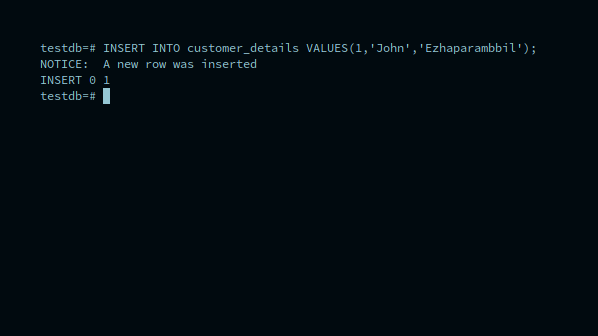
\includegraphics[width=\linewidth]{../Images/Triggers/1.png}

	\item Create a trigger to display a message when a user enters a value greater than 20000 in the salary field of emp\_details table.
	\begin{verbatim}

	CREATE OR REPLACE FUNCTION log_sal_changes()
	  RETURNS trigger AS
	$$
	BEGIN
		IF NEW.salary > 20000 THEN
	  	RAISE NOTICE 'Employee has salary greater than 20000/-';
		END IF;
		RETURN NEW;
	END;
	$$ LANGUAGE plpgsql;

	CREATE TRIGGER salary_changes
	  BEFORE INSERT
	  ON emp_details
	  FOR EACH ROW
	  EXECUTE PROCEDURE log_sal_changes();


	\end{verbatim}
	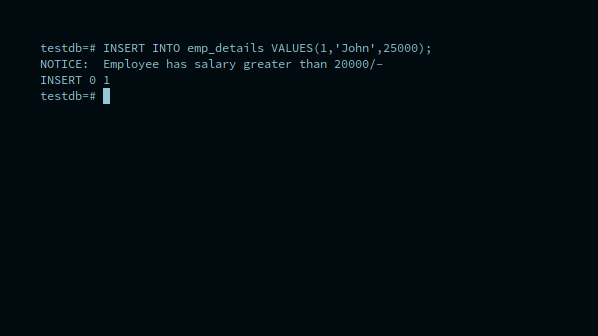
\includegraphics[width=\linewidth]{../Images/Triggers/2.png}

	\item Create a trigger w.r.t customer\_detailstable.Increment the value of count\_row (in cust\_count table) whenever a new tuple is inserted and decrement the value of count\_row when a tuple is deleted. Initial value of the count\_row is set to 0.
	\begin{verbatim}
	
CREATE OR REPLACE FUNCTION update_count()
	RETURNS trigger AS
$$
BEGIN
	UPDATE cust_count SET count_row = (SELECT count(*) FROM customer_details);
	RETURN NEW;
END;
$$ LANGUAGE plpgsql;

CREATE TRIGGER count_changes
	AFTER INSERT OR DELETE
	ON customer_details
	FOR EACH ROW
	EXECUTE PROCEDURE update_count();

	\end{verbatim}
	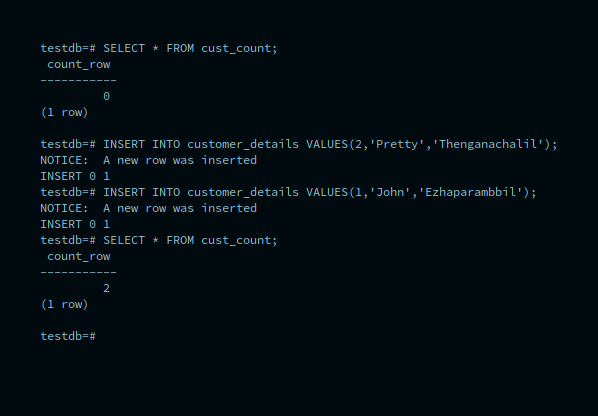
\includegraphics[width=\linewidth]{../Images/Triggers/3.png}
	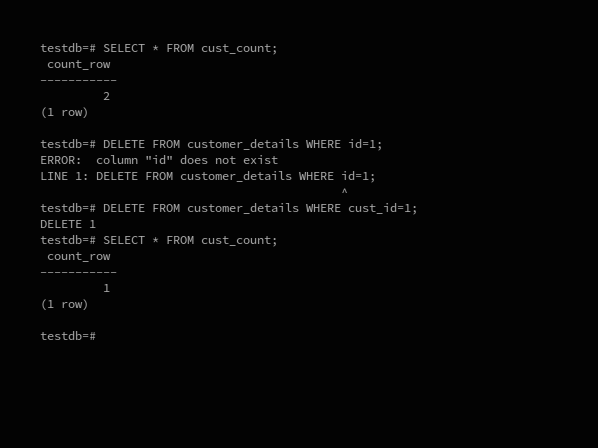
\includegraphics[width=\linewidth]{../Images/Triggers/8.png}

	\item Create a trigger to insert the deleted rows from emp\_details to another table and updated rows to another table.(Create the tables deleted and updated)
	\begin{verbatim}
CREATE OR REPLACE FUNCTION archive_deleted()
	RETURNS trigger AS
$$
BEGIN
	INSERT INTO deleted VALUES(OLD.*);
	RETURN NEW;
END;
$$ LANGUAGE plpgsql;

CREATE OR REPLACE FUNCTION archive_updated()
	RETURNS trigger AS
$$
BEGIN
	INSERT INTO updated VALUES(OLD.*);
	RETURN NEW;
END;
$$ LANGUAGE plpgsql;

CREATE TRIGGER archive_deleted_trig
	BEFORE DELETE
	ON emp_details
	FOR EACH ROW
	EXECUTE PROCEDURE archive_deleted();

CREATE TRIGGER archive_updated_trig
	BEFORE UPDATE
	ON emp_details
	FOR EACH ROW
	EXECUTE PROCEDURE archive_updated();

	\end{verbatim}
	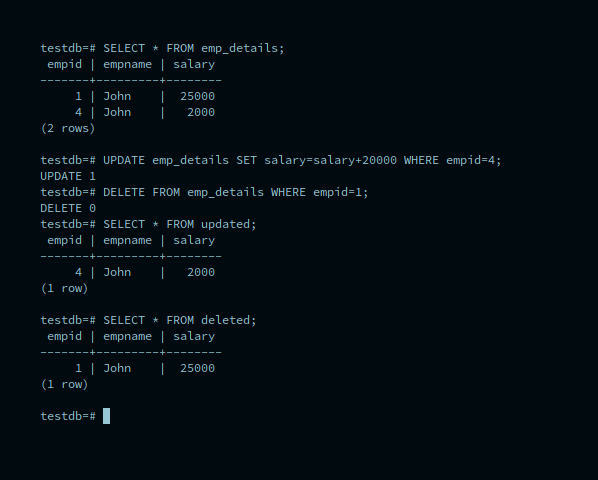
\includegraphics[width=\linewidth]{../Images/Triggers/4.png}

	\item Write a PL/SQL to show divide by zero exception
	\begin{verbatim}
CREATE OR REPLACE FUNCTION divide(a REAL, b REAL)
RETURNS REAL AS
$$
BEGIN
  IF b = 0 THEN
    RAISE EXCEPTION 'Division by Zero';
    RETURN null;
  ELSE
    RETURN a / b;
  END IF;
END;
$$ LANGUAGE plpgsql;

	\end{verbatim}
	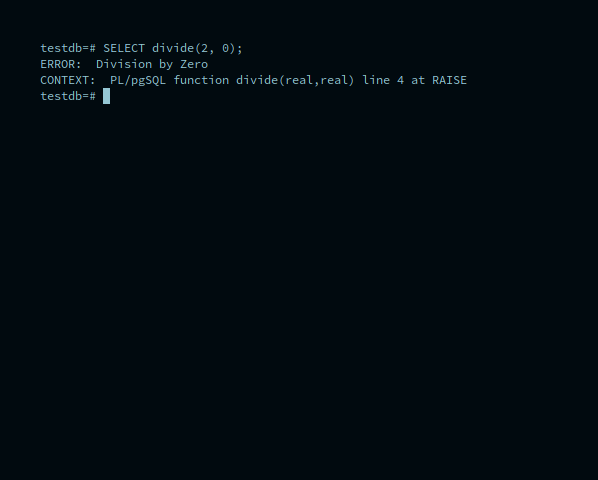
\includegraphics[width=\linewidth]{../Images/Triggers/5.png}

	\item Write a PL/SQL to show no data found exception
	\begin{verbatim}
CREATE OR REPLACE FUNCTION func_ex() RETURNS trigger AS
$$
DECLARE
  var_name name;
BEGIN
WHEN NO_DATA_FOUND THEN RAISE EXCEPTION 'No data found. Try another query.';
RETURN NEW;
END;
$$ LANGUAGE plpgsql;
CREATE TRIGGER insert_trigger AFTER UPDATE ON people_list EXECUTE PROCEDURE func_ex();

	\end{verbatim}
	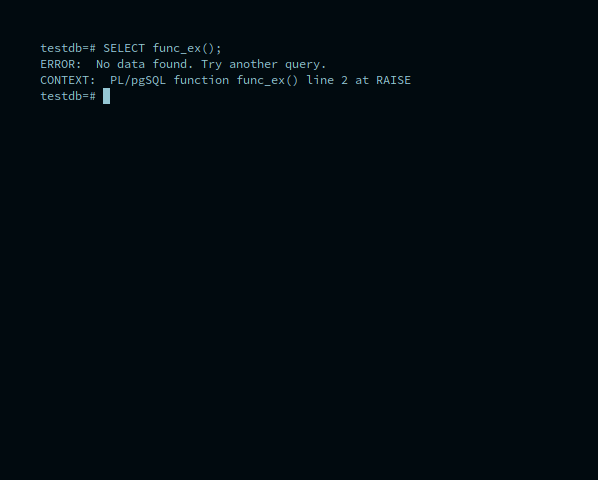
\includegraphics[width=\linewidth]{../Images/Triggers/6.png}


	\item Create a table with ebill(cname,prevreading,currreading). If prevreading = currreading then raise an exception ‘Data Entry Error’.
	\begin{verbatim}
CREATE OR REPLACE FUNCTION check_bill()
RETURNS TRIGGER AS
$$
BEGIN
  IF NEW.prevreading = NEW.currreading THEN
    RAISE EXCEPTION 'Data Entry Error';
    RETURN OLD;
  ELSE
    RETURN NEW;
  END IF;
END;
$$ LANGUAGE plpgsql;

CREATE TRIGGER bill_check
	BEFORE INSERT
	ON ebill
	FOR EACH ROW
	EXECUTE PROCEDURE check_bill();

\end{verbatim}

	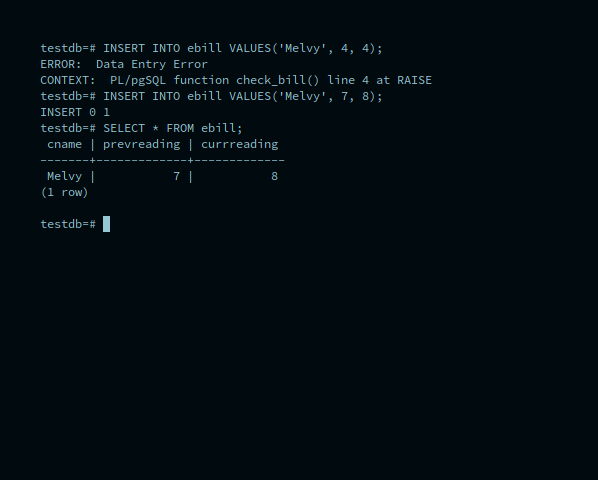
\includegraphics[width=\linewidth]{../Images/Triggers/7.png}
\end{enumerate}

\subsubsection{RESULT}
The PL/SQL programs were executed successfully and the output was obtained.

}
\end{document}
